\section{Problem 5}
\label{part5}
\subsection*{Question}
\begingroup
\begin{verbatim}
5.  Re-run question 2, but this time with proper TFIDF calculations
instead of the hack discussed on slide 7 (p. 32).  Use the same 500
words, but this time replace their frequency count with TFIDF scores
as computed in assignment #3.  Document the code, techniques,
methods, etc. used to generate these TFIDF values.  Upload the new
data file to github.

Compare and contrast the resulting dendrogram with the dendrogram
from question #2.

Note: ideally you would not reuse the same 500 terms and instead
come up with TFIDF scores for all the terms and then choose the top
500 from that list, but I'm trying to limit the amount of work
necessary.
\end{verbatim}
\subsection{Answer}
\begin{enumerate}
\item I used the python which is used to get the matrix for the questions $1$ but added few lines of code to calculate the TFIDF value for each word
\item IDF value is calculated at line 149 in Listing \ref{lst:tfidf}  
\item The TF value for each word with respective to each blog is calculated at line 166 which is used to calculate TFIDF value at line 167 in Listing \ref{lst:tfidf}
\item The matrix with blog name and the words along with their TFIDF value is calculated by The program Listed in Listing \ref{lst:tfidf}. The output is uploaded in the github as \emph{bloglist-500-matrix.txt}.
\item I used the same program which I used in Problem 2 to generate the dendrogram shown in Figure \ref{fig:q5dendrogram}

\item Unfortunately, it is difficult to see, but this dendogram shows that the blogs calculated to be most like \emph{F-Measure} are split into two clusters, the blogs in the first cluster is \emph{Music Liberation} contrast to the out from the dendrogram from the second question the blog \emph{/YOUNGEST INDIE}
\item The blogs in second cluster are \emph{YOUNGEST INDIE} and \emph{McCrak's Juke} where as the the blog \emph{The Devil's Music} is in the second cluster instead of \emph{YOUNGEST INDIE} in the dendrogram produced for second question .

\item Unlike in the dendrogram produced for the second question The blog calculated to be most like \emph{Web Science and Digital Libraries Research Group} is \emph{Buckaroo's Bazar}

\item From my observation of both the dendrograms I found that the hierarchy of the clusters are changing but somehow that clusters are around the same blogs with different hierarchy. 
\item The accuracy of matching the most alike blogs is changing.
\end{enumerate}

\subsection{Output for 5th problem}

\begin{figure}[h]
\centerline{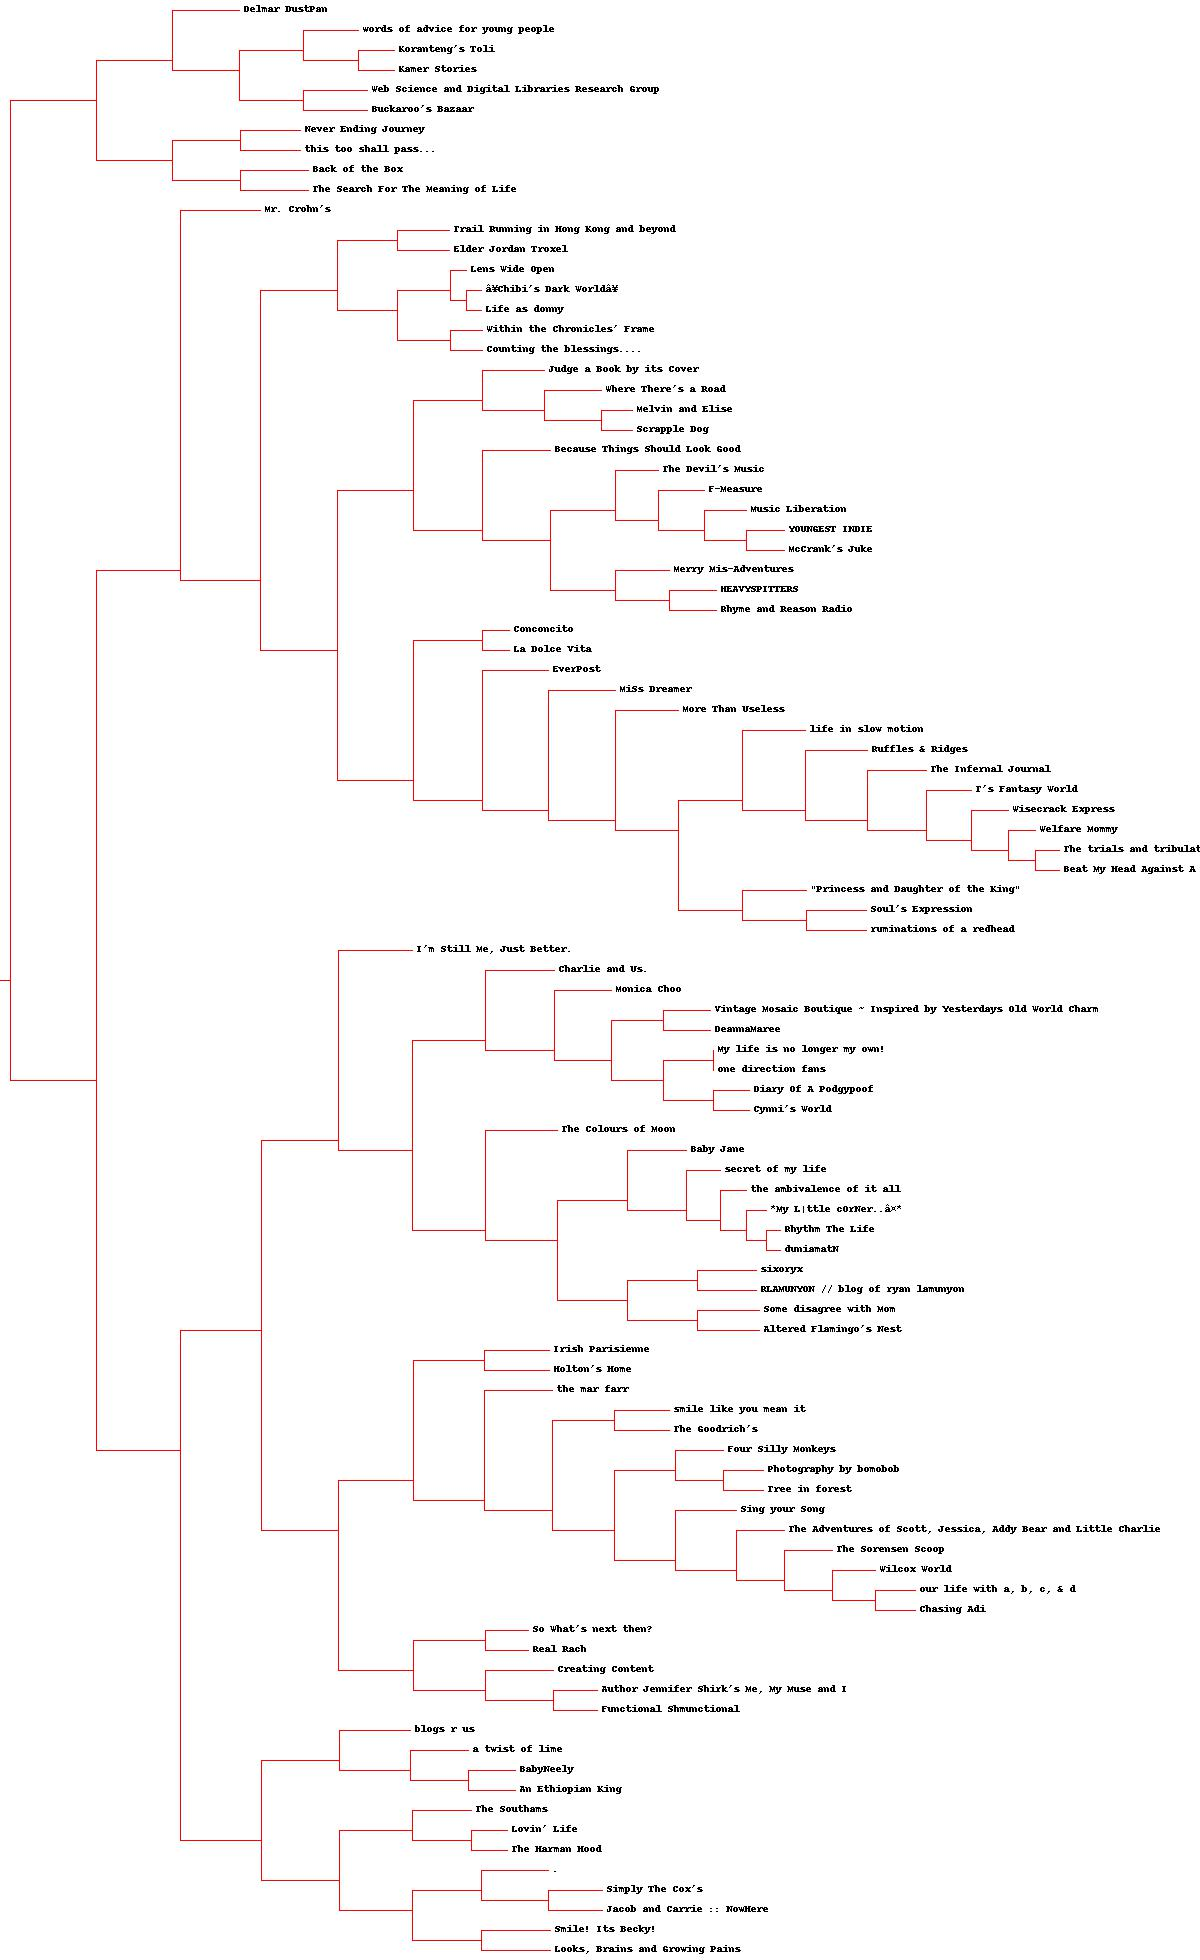
\includegraphics[scale=0.36]{questions/q5/blogclust-q5.jpg}}
\caption{Dendrogram produced based on word's TFIDF values script}
\label{fig:q5dendrogram}
\end{figure}

\newpage

\lstinputlisting[language=python, frame=single,breaklines=true, caption={Python code for grabbing popular 500 words from 100 atom feeds and their TFIDF values},captionpos=b, numbers=left, showspaces=false,label=lst:tfidf, showstringspaces=false, basicstyle=\footnotesize]{questions/q5/tfidf.py}



\newpage
\lstinputlisting[frame=single,
caption={Segaran's \emph{clusters.py}},label=lst:clusters,
captionpos=b,numbers=left,showspaces=false,
showstringspaces=false,basicstyle=\footnotesize]{questions/q2/clusters.py}